\chapter{State of the art}
\label{sec:stateoftheart}

%\footnote{The name of this thesis is about processing of medical information. Processing of any type of information might be done using local PC. The processing might take a lot of time thus it's desirable to perform processing on some more powerful hardware: workstation, server, cluster of servers.}

Processing of medical information deals with methods that connects different scientific domains, computer science, biomedical engineering and medicine together with a common goal. 

%Medical informatics, computational biology, bioinformatics}
Medical informatics (MI) deals with informatics methods used in clinical medicine and healthcare. While bioinformatics (BI) focus more on development and application of new informatics techniques in biological (mainly genomic) sciences. Computational Biology (CB) study the biological systems formalized as mathematical models and using computational methods to simulate and compare with real systems. Recent development in the fields joined a scientific effort to translate the successful techniques into clinical medicine and helathcare as well as to improve other scientific disciplines.
Maojo et al. \cite{Maojo2003} and Martin-Sanchez et al.\cite{Martin-Sanchez2004} described relationship between MI and BI and within the new field of Biomedical informatics.

In further chapters all aspects will be touched, the bioinformatics approach to develop new techniques, biomedical approach to deliver such techniques to clinical use as well to the basic research  computational biology approach to do basic science.


From computer science point of view, it is assumed that a processing of medical information is in general a computational problem which is understood as a task that can be solved by a computer. 

Because some computationally hard problems will be touched in further text whose exact solution need tremendous amount of time or space, therefore next sections introduces briefly theoretical and practical aspects of computation, parallelism, distributed computing. Section \ref{sec:introcomplexity} introduces some important problem classes from the view of computational complexity theory. 

Parallel computation may introduce in some condition speedup needed for computing complex problems, the theory is covered briefly in section \ref{sec:introparalel}.

Distribution of parallel task via computer network to another computers, servers and clusters is covered in section \ref{sec:distributed} with focus on grid-computing and cloud-computing.

\section{Computational complexity}
\label{sec:introcomplexity}

An algorithm is a set of operation to acomplish the task and solve the problem. There are several ways howto express algorithm, e.g. in text in programming language or pseudocode or flowcharts are used. In further text the kopenograms will be used as graphical language for structured algorithms to supplement UML proposed by Kofranek et al.\cite{Kofranek2012}\footnote{\url{http://www.kopenogram.org} accessed March 2015}.

The computational complexity theory studies and classifies problems into several classes according to the time or space needed by the algorithm solving the problem.

Time complexity of an algorithm is usually denoted by big $O$ notation defined for function $f$ and $g$ and size of input data $n$ that 
$f(n)=O(g(n)$ if $f$ is not growing faster than $g$. Formally $f(n)=O(g(n)$ if and only if there exists constant $c$ and positive integer $n_0$ that for each $n\geq n_0$: $f(n) \leq c \times g(n)$

$O(1)$ usually denotes algorithms that takes constant time regardless of size of the input. $O(n)$ denotes algorithms that takes time is linear. E.g. sequential search algorithm in fig.\ref{fig:search} need to compare each record with a given key and is used to find some item in an unsorted list or array. Single comparison takes e.g. $0.03$ seconds and list has $n$ records, then algorithm will take at worst $n$ steps and time complexity is $f(n) = 0.03 \cdot n = O(n)$. A better approach is usually achieved with B-tree data structure holding sorted list of records and binary search algorithm applied on this data structure takes logaritmic time complexity $O(\log(n))$ which is better than the previously introduced sequential algorithm \cite{Bayer1972Org,Bayer1972Sym}.

\begin{figure}[ht]
    \centering
    \includegraphics[page=3]{chapter3/GA-kopenogram-crop.pdf}    
%    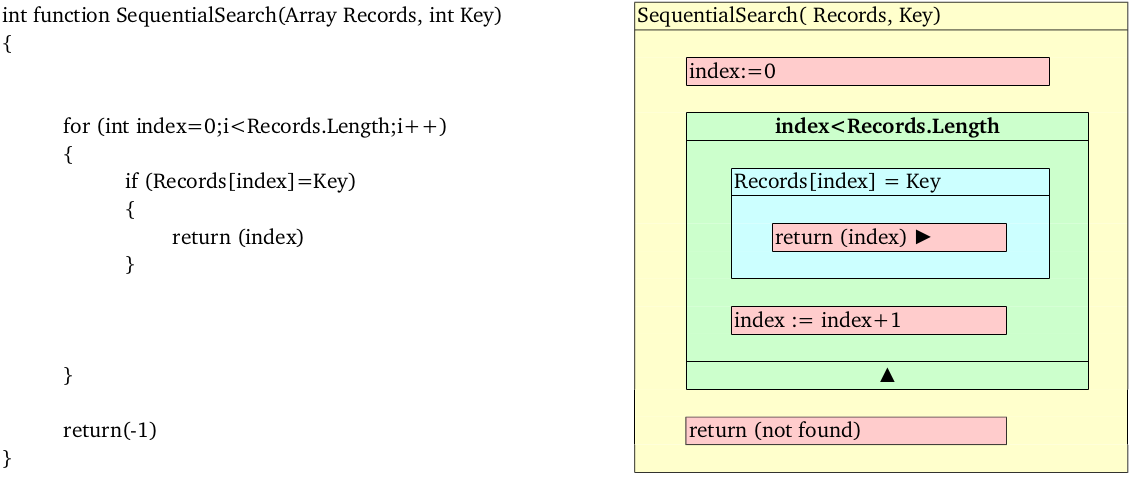
\includegraphics[width=1\textwidth]{chapter2/seqsearchkopenogram.png}
    \caption{Pseudocode (left) and kopenogram (right) of sequential search algorithm with complexity $O(n)$. The red blocks are commands, i.e. setting the index or returning results. The green block represents the loop with entry condition. The index is incremented and in programming languages this can be done e.g. by \emph{for} cycle statement. The blue block is condition (\emph{if} statement), when fulfilled then the inner blocks are executed, in our case the found index is returned. If no record is found, the loop will end with the last index within \emph{Records} and \emph{not found} sign is returned. }
    \label{fig:search}
\end{figure}

Polynomial time algorithms are defined as the one which time complexity can be bounded by $O(n^k)$ for some constant $k$. Class of problems which are solvable by polynomial algorithm are denoted as \emph{class P} and are recognised as tractable\cite{Cobham1964,Cook1983} and other algorithms whose time cannot be bounded by any polynomial function are called exponential and are recognised as intractable \cite{Garey1979,Cook1983}. 

E.g. brute-force search is general solving technique that generates all possible candidates of solution and checks if the problem satisfies the problem statement. All the algorithms to solve brute-force search suffers with exponential time complexity$O(k^n)$ even e.g. depth-first iterative-deepening algorithm for brute-force search was shown to be optimal compared to other standard brute-force search algorithm (depth-first search or breadth-first search)\cite{Korf1985,Pearl1987}.

In the past there were identified several class of problems, for which the current 
%For the class of \emph{NP-complete} problems (non-deterministic polynomial, where if some guess is provided, it can be verified in polynomial time whether it is the solution or not) the current 
best known algorithm is based on brute-force search of all possible values and better does not exists, or it is open question whether it exists. E.g. For the class of {NP-complete} problems if a polynomial algorithm will be discovered for one problem of this class in future, it was shown that all other NP-complete problems would be solvable by a polynomial algorithm derived from the discovered one\cite{Cook1971,Karp1972}.

The analysis of complexity of algorithms and problems mentioned above is important for further consequences on computability.
For a relatively small input data the exact solution can be found using the known exponential algorithm with current computation power, however, for bigger input data the time needed to solve the problem is far beyond reasonable amount as seen from Table \ref{table:timecomplexity}.
\begin{table}[ht]
\footnotesize
\begin{tabular}{|l|r|r|r|r|}
\hline
\diagbox[height=43pt,width=125pt]{time\\complexity\\function}{input size \\ $n$} & 10          & 20        & 50             & 100            \\ \hline
$n$                                                                           & $00.01$ s     & $00.02$ s   & $00.05$ s        & $00.10$ s        \\ \hline
$n^2$                                                                         & $00.10$ s     & $00.40$ s   & $02.50$ s        & $10.00$ s        \\ \hline
$n^5$                                                                         & $01$m $40.00$ s & $53$ m $20$ s & $14$h $48$m $20$s    & $116$ days       \\ \hline
$2^n$                                                                         & $01.02$ s     & $17$ m $28$ s & $35702$ years    & $4.02\times 10^{19}$ years \\ \hline
$3^n$                                                                         & $59.05$ s     & $40$ days   & $2.28\times 10^{13}$ years & $1.63\times 10^{37}$ years \\ \hline
\end{tabular}
\caption{Computation time of algorithms with different time complexity functions, where one step of algorithm takes 1 milisecond. Examples of algorithm with polynomial time complexity $O(n^k)$ are compared with algorithm with exponential time complexity $O(k^n)$. Note that for the problems with input size of 50 and greater the exponential algorithm runs far beyond the reasonable time compared to the age of universe which is currently estimated to $13.8\times 10^9$  years \cite{PlanckCollaboration2013}.}
\label{table:timecomplexity}
\end{table}

If we presume technological update and the computation speed will increace, the effect of technological speedup is visible in table \ref{table:speedupeffect}. The effect on polynomial algorithm is multiplicative, however for exponential algorithm, the technological speedup will increase the size of computable problem only slightly, this is reason why the problems which best algorithms has exponential complexity are denoted as intractable. 
\begin{table}[ht]
\footnotesize
\begin{tabular}{r|c|c|c|c|}
                      & present computer   & 10 times faster               & 100 times faster               & 1000 times faster \\
\hline
\multirow{2}{*}{$n$}  & 3600000        & 36000000         & 360000000        & 3600000000      \\
                      & $1\times$          & $10\times$   & $100\times$  & $1000\times$ \\
\hline
\multirow{2}{*}{$n^2$}                 & 1897 & 6000             & 18973 & 60000            \\
                      & $1\times$          & $3.16\times$ & $10\times$   & $31.6\times$ \\
\hline
\multirow{2}{*}{$n^5$}                 & 20  & 32     & 51    & 81    \\
                      & $1\times$          & $1.59\times$ & $2.51\times$ & $3.98\times$ \\
\hline
\multirow{2}{*}{$2^n$}                 & 21  & 25    & 28    & 31    \\
                      & $N_{2^n}$       & $N_{2^n}+3.32$    & $N_{2^n}+6.64$    & $N_{2^n}+9.97$    \\
\hline
\multirow{2}{*}{$3^n$} & 13  & 15    & 17    & 20    \\
                      & $N_{3^n}$       & $N_{3^n}+2.09$    & $N_{3^n}+4.19$     & $N_{3^n}+6.29$                  \\
                      \hline
\end{tabular}
\caption{ Effect of computation speedup. First value is input size of data computable in one hour, second value is speedup achieved compared to the value in first column. }
\label{table:speedupeffect}
\end{table}

%Note that the age of universe is currently estimated to $13.8\times 10^9  years$ \cite{PlanckCollaboration2013}.
NP-complete problems (currently exponential algorithm can solve them and it was not found better algorithm) are covered in book of M. R. Garey and D. S. Johnson \cite{Garey1979}. The whole complexity theory is covered e.g. in book by Ch.Papadimitriou \cite{Papadimitriou1995} or in a book by M.Sipser \cite{Sipser2012}. 

To summarize this section. If there will be technological speedup, this will impact mainly the class of problems which are solvable by polynomial algorithm. For the problems where the computation needs tremendous ammount of time, because current known algorithm is exponential, there can be used non-exact methods to find at least some solution if not the exact one. 
\begin{itemize}
\item{The \emph{heuristic methods} tries to eliminate the number of steps of computation by some implicit or explicit knowledge of the specific problem itself E.g. eliminating solution classes that seems not to go to optimal solution. With combination of brute-search the heuristic methods reduce the size of all possible solution candidates to check.}
\item{The \emph{randomization methods} use non-deterministic methods in some level of computation.E.g. Monte-Carlo method is used to compute problems using pseudo-random generated values and after several iterations statistical methods are used to compute expected value and standard deviation. }
\item{\emph{Restriction on input data} - is another form of using the explicit knowledge of the problem instance ad it may reduce all possible values to be checked. }
\item{\emph{Approximation algorithm} - may find not only some good solution, but can quantify how far from the optimal solution the found is good with some degree of probability.}
\end{itemize}


\section{Parallelization}
\label{sec:introparalel}

If a sequence of instructions can be divided into parts which  can be computed independently in parallel by multiple processors, then it is possible to achieve some computation speedup using current computational technology. %Parallel computing can be utilized in several types of application which are further distinguished by the types of location and access to the computation resources. 

We can define a speedup of a computation on P processors as follows:
\begin{equation}\label{eq:speedup}
 S(P) = \frac{\text{time on 1 processor}}{\text{time on P processors}}
 \end{equation}

We can estimate speedup of an computation of a fixed-size problem and then we can ask how can we speedup this problem on P processor. In fig. \ref{fig:serialvsparallel} is example of serial and parallel computation of the same problem.

\begin{figure}[ht]
    \centering
    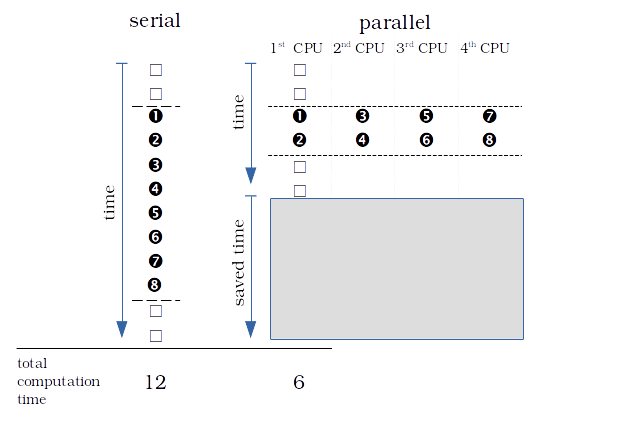
\includegraphics[width=1\textwidth]{serialvsparallel.png}
    \caption{Comparison of serial and parallel processing of instructions, the instructions which can be computed in parallel are with numbers. In this case the serial computation takes 12 cycles, parallel computation on 4 CPU takes 6 cycles. The speedup is $2$ times. If we have 8 CPUs, then a computation will be finished in 5 cycles and the speedup will be $2.4$ times.}
    \label{fig:serialvsparallel}
\end{figure}

Assume  $\alpha \in (0,1)$ as a fraction of the computation in one processor which cannot be parallelized, $(1-\alpha)$ is fraction of the computation in one processor which can be parallelized by $P$ processors and $t$ is time needed to compute the process on one processor. Assume that overhead of parallelization is small and can be disregarded. Then speedup can be computed as:
\begin{equation}\label{eq:speedup2}
 S(P) = \frac{t\times\alpha+t\times(1-\alpha)}{t \times \alpha + \frac{t \times (1-\alpha)}{P} } = \frac{1}{\alpha +\frac{1-\alpha}{P}}
 \end{equation}
On unlimited number of processors it can be formulated theoretical upper bound of speedup which depends on $\alpha$ only:
\begin{equation} \label{eq:amdahl}
S = \lim_{P \to \infty} \frac{1}{\alpha +\frac{1-\alpha}{P}} = \frac{1}{\alpha}
\end{equation}

This is recognized as Amdahl's law \cite{Amdahl1967}. E.g. when a 10\% of computation cannot be parallelized( $\alpha = 0.1$) then the speedup on 10 processors can be $S(P) = \frac{1}{0.1+0.9/10} = 5.26$ and theoretical speedup on unlimited number of processors is $S = 1/0.1=10$. See more at fig \ref{fig:amdahl}.
\begin{figure}[ht]
    \centering
    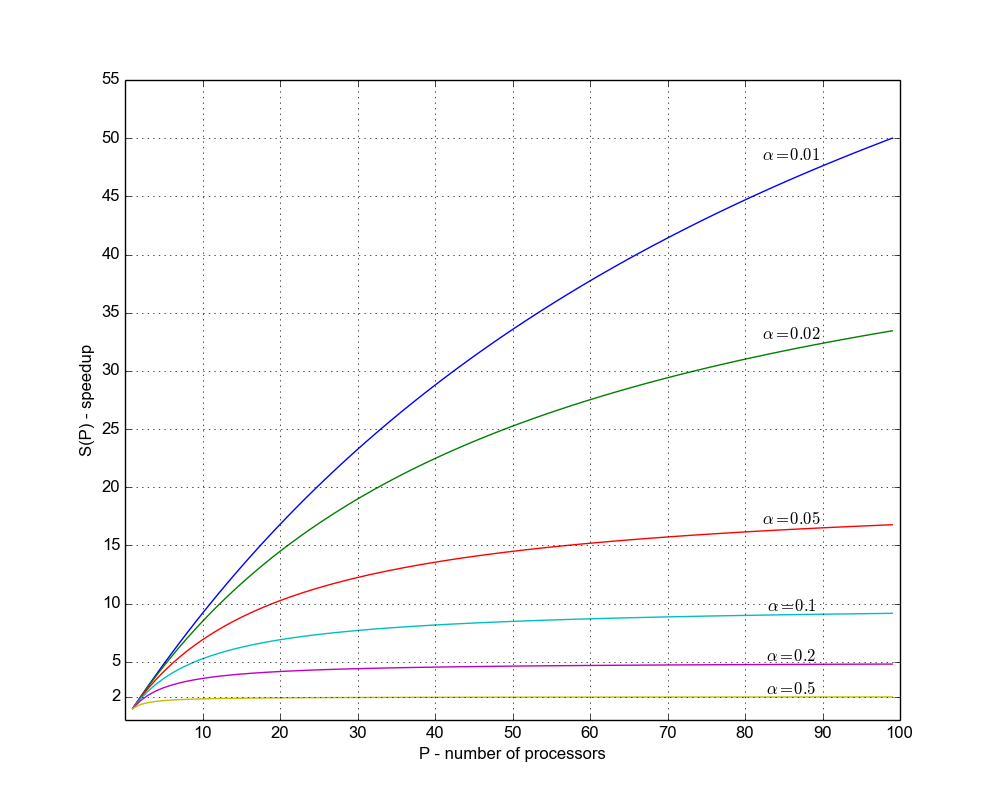
\includegraphics[width=1\textwidth]{chapter2/Amdahl.png}
    \caption{Speedup gained on 1 to 100 processors per Amdahl's law for different $\alpha$ values.}
    \label{fig:amdahl}
\end{figure}

However, $\alpha$ could be sometimes hard to estimate and computing the fixed size problem on high number of processors can misrepresent the speedup and performance discrepancy. Therefore, Gustafson reformulated the law and described another approach. Measure the fraction of the computation which cannot be parallelized from computing on $P$ processors and estimate the speedup from how long will such computation take on single processor. Assume that overhead of parallelization is small and can be disregarded. The $\beta$ is "scaled fraction" of computation on $P$ processors which cannot be parallelized \cite{Gustafson1988}:
\begin{equation} \label{eq:gustafson}
S(P) = \frac{t \times \beta + t\times(1-\beta)\times P}{t\times\beta+t\times(1-\beta)} = \beta + (1-\beta)\times P 
\end{equation}
This law presumes that the fraction $\beta$ will not change on different number of processors, as seen at fig \ref{fig:gustafson}.
\begin{figure}[ht]
    \centering
    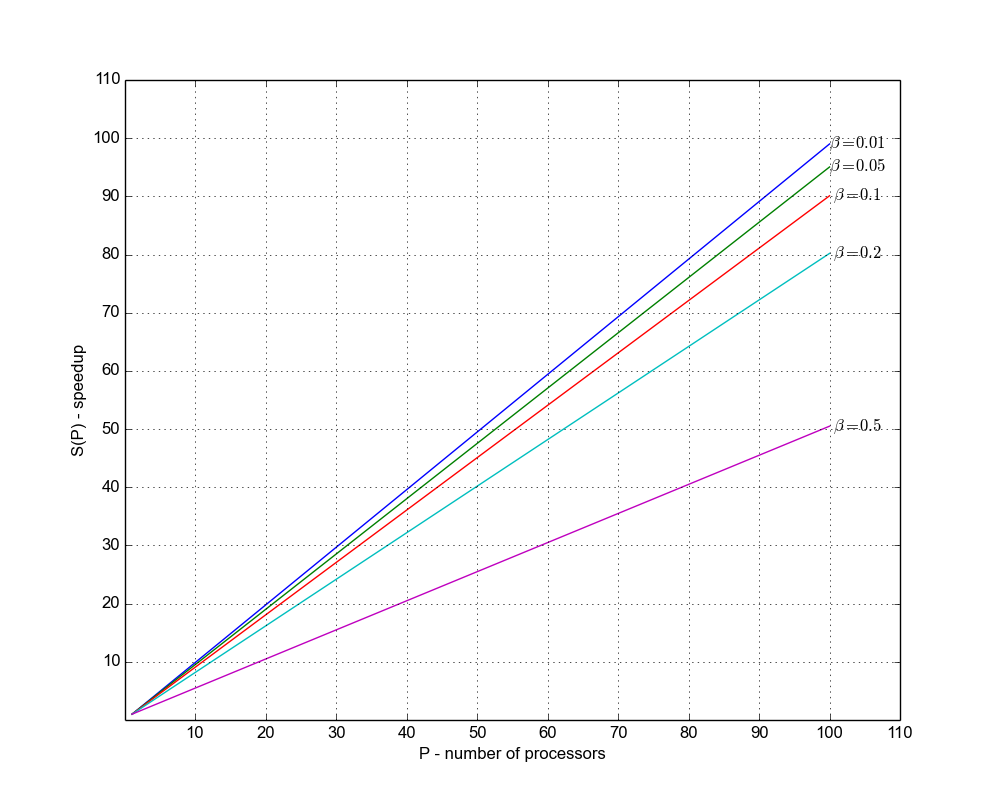
\includegraphics[width=1\textwidth]{chapter2/Gustafson.png}
    \caption{Speedup gained on 1 to 100 processors per Gustafson's law for different $\beta$ values.}
    \label{fig:gustafson}
\end{figure}

Both laws disregard parallelization overhead, however if there is significant one, the speedup of parallelization will be degraded by the overhead. The Amdahl's law (\ref{eq:amdahl}) is argument that the speedup is limited for current sized problem, however, bigger problems can be addressed with higher number of processors and this should be considered with regard to Gustafson's law (\ref{eq:gustafson}).

\subsection{Programming model}
\label{sec:parallelprogramming}
Looking into how the parallelization is realized, there are several levels of parallelism.
\begin{itemize}
\item{\emph{Instruction level parallelism} - instructions of a program can be executed at the same time, if they are independent. Programs are usually written as a sequence of instruction and it depends on compiler capability to recognize or reorder the instruction so some set of instruction can be executed by a specific processor in parallel. Instruction parallelism started to be systematically utilized in multi-core processor.}
\item{\emph{Data parallelism} - the same operation is performed on multiple data, usually arrays. The instruction is distributed into multiple processors or processor cores and is executed on elements of data structure in parallel. This is currently characteristic feature of \emph{General purpose graphical processing unit}(GPGPU) computing and heterogenoust programmable API such as CUDA\footnote{\url{https://developer.nvidia.com/cuda-zone} accessed February 2015} and OpenCL\footnote{\url{https://www.khronos.org/opencl/} accessed February 2015}}
\item{\emph{Loop parallelism} - the computation may contain a iterative processing of a large data structure. Usually such iterative processing is programmed as a loop and if $i^{th}$ iteration is independent on $(i-1)^{th}$ then the iteration can be executed in parallel by different processors.}
\item{\emph{Task parallelism} - the computation contains parts which are independent of each other. Computation of such parts can be scheduled and distributed into multiple processors and can be computed concurrently. Typical Master/Worker pattern is realized(master sets up a pool of worker processed and a set of tasks which is distributed to them). Fork/Join pattern - main process forks into several threads executing concurently and waits for their results to join back into a single process which may after some computation again fork.}
\end{itemize}

Looking into the way how the processes interacts, these are the most common forms:
\begin{itemize}
\item{The \emph{threads} are several concurent execution paths which are independent, but in general share the same memory. It was standardized e.g. as a POSIX threads  (Pthreads) and are implemented by standard C libraries in different platforms\cite{Butenhof1997}.}
\item{\emph{shared memory}. The \emph{OpenMP}\footnote{\url{http://openmp.org/} accessed February 2015} is a shared memory application interface standardized and implemented in by several compilers for C, C++ and Fortran. It uses also multithreaded model, however programming is task oriented and more abstract\cite{Chapman2008}. }
\item{\emph{message passing}. The \emph{Message Passing Interface}(MPI) is specification for message passing between tasks. This is usually used, when tasks doesn't share the memory \cite{Pacheco1997}.
}
\end{itemize}
More about parallel programming models can be found in survey by Diaz et al. \cite{Diaz2012}.
\subsection{Summary}

Some algorithms can be divided easily into independent tasks, which can be computed in parallel. If there is no need to communicate among the parallel tasks, such algorithms are called embarrassingly parallel. E.g. 
\begin{itemize}
\item{Operation on matrices  \cite{Moler1986} are currently used to render 2D and 3D graphics.}
\item{Parameter study, where the same computation is performed using different set of input parameters \cite{Foster1995}.}
\item{Brute-force search algorithm, where subset of possible candidates for solution are generated and checked in parallel.}
\item{Genetic algorithm and other evolutionary algorithms \cite{Cantu-Paz1999}.}
\end{itemize}
In contrast to embarrassingly parallel problems, the opposite are algorithms that are inherently sequential or are believed that cannot be significantly speeded up by parallel computing. The theory about this problems and related algorithm which are denoted as problems/algorithm in class \emph{P-complete} are believed not to get significant speedup using parallel computing, see e.g. book of Greenlaw et al. \cite{Greenlaw1995}. 

The same problem can be solved by different algorithms with different scalability (how they can be speed up by parallel computing) and different effectivity (what is the time complexity) and these both aspects should be considered together \cite{Madden2012}. 

Further aspects of parallel computing can be found in the book of D.Culler et al  \cite{Culer1998}, book of T.Rauber and G.Räuder \cite{Rauber2013} or earlier book about design and build parallel programs of I.Foster  \cite{Foster1995}.

To summarize this section; parallel computing can introduce speedup on current computational technology and some computation problems may become feasible.
Also overhead caused by parallelization and fraction of non-parallelizible parts should be considered as it may degrade expected speedup.
In case of exponential algorithm (e.g. for NP-complete problems) the speedup will increase the size of solvable problem only slightly (see table \ref{table:speedupeffect}) and some problems cannot be (or it is believed) significantly speedup by parallel computing. 
In further text a focus will be given mainly to task parallelism and distributed computing. 

\section{Distributed computing technologies}
\label{sec:distributed}

%An important idea is to share computational resources among multiple different users and communities. Several issues needs to be addressed e.g. authentication and authorization using security protocols and database of privileges. Other is scheduling, thus the work of all potential users will not collide in one time and in another time the resources will not be utilized. 
Distributed computing is based on the idea to spread the computation task into set of computers which are connected via computational network.

Main motivation of using distributed computing technologies are (1) sharing, storing and exchanging data (2) provide and consume computational services (3) access the much higher capacity of storage and computation than available locally.

To manage distributed computing several challenges are maintained such as synchronization(exchange of messages in computation workflow) to achieve e.g. mutual exclusion(when a task needs exclusive access to some resource) and prevent deadlock(no progress is possible) or resource starvation(when a resources - e.g. processor time - is not scheduled for particular task for some reasons and task cannot finish it's computation). Distributed systems offer some sort of fault tolerance (managing fault of a node during computation) or security (encryption of communicating channels and stored data, authentication and authorization to access some resources or data) etc. The topic of distributed computing is covered e.g. in book of Tannenbaum \cite{Tanenbaum2007}. 

An extreme example of distributed computing is Internet where the computers are interconnected via TCP/IP protocols, the services are provided by servers (e.g. web servers) with some degree of security and fault tolerance. E.g. world wide web is based on HTTP protocol and HTML language and related technologies, peer to peer services are based on TCP/IP or UDP and streaming of data.

For scientific purposes, the distributed computing infrastructures evolved into set of clusters, computing centers or individual computing resources owned by different subjects. And an effort is continuously done to join such resources into a federation of computational capacity via high speed network to obtain optionally better virtual capacity in case of need. There were formulated some minimal requirements and defined and implemented standards for network protocols and services that a distributed infrastructure should fulfil and provide. Such infrastructures are currently distinguished as grid-computing or cloud-computing infrastructures and the users of it can get access to much higher virtual capacity than accessible locally. Users also may access remotely specialized devices which are not available within their institution.

%\subsection{Software architecture}
%\label{sec:introintegration}
\subsection{Programming model}
\label{sec:distributedprogramming}

When we look how the distributed computing is realized, the parallel programming model (section \ref{sec:parallelprogramming}) is used and additionally higher level of task interaction is realized via shared distributed file system or messages passed over computer network. 
Looking into the software layers, distributed computing incorporates usually one or several new layers. Middleware is a software which delivers services or APIs for application and hides specific implementation across heterogenous computing platforms(operating system and hardware).

\subsubsection{System Architecture}

As the algorithms and programs needed to solve increasing number of problems and changing requirements, the systematic approach and order in several programs and algorithms is adopted to constructing robust software system which will solve the complex problems -- software architecture.

The decision about software architecture are made at the begining of a project and are hard to change in implementation is influenced by the experiences that building an application and solution from scratch is too expensive and time consuming. Integrating non-compatible modules might be also time consuming therefore several architecture paradigmas, constraints and patterns are followed to facilitate joining different blocks of software to complex system solving complex problems.

The major software architecture within distributed computing are based on client-server architecture (Example in fig. \ref{fig:architecture}), peer-to-peer architecture or more layered architecture patterns.
\begin{figure}[ht]
    \centering
    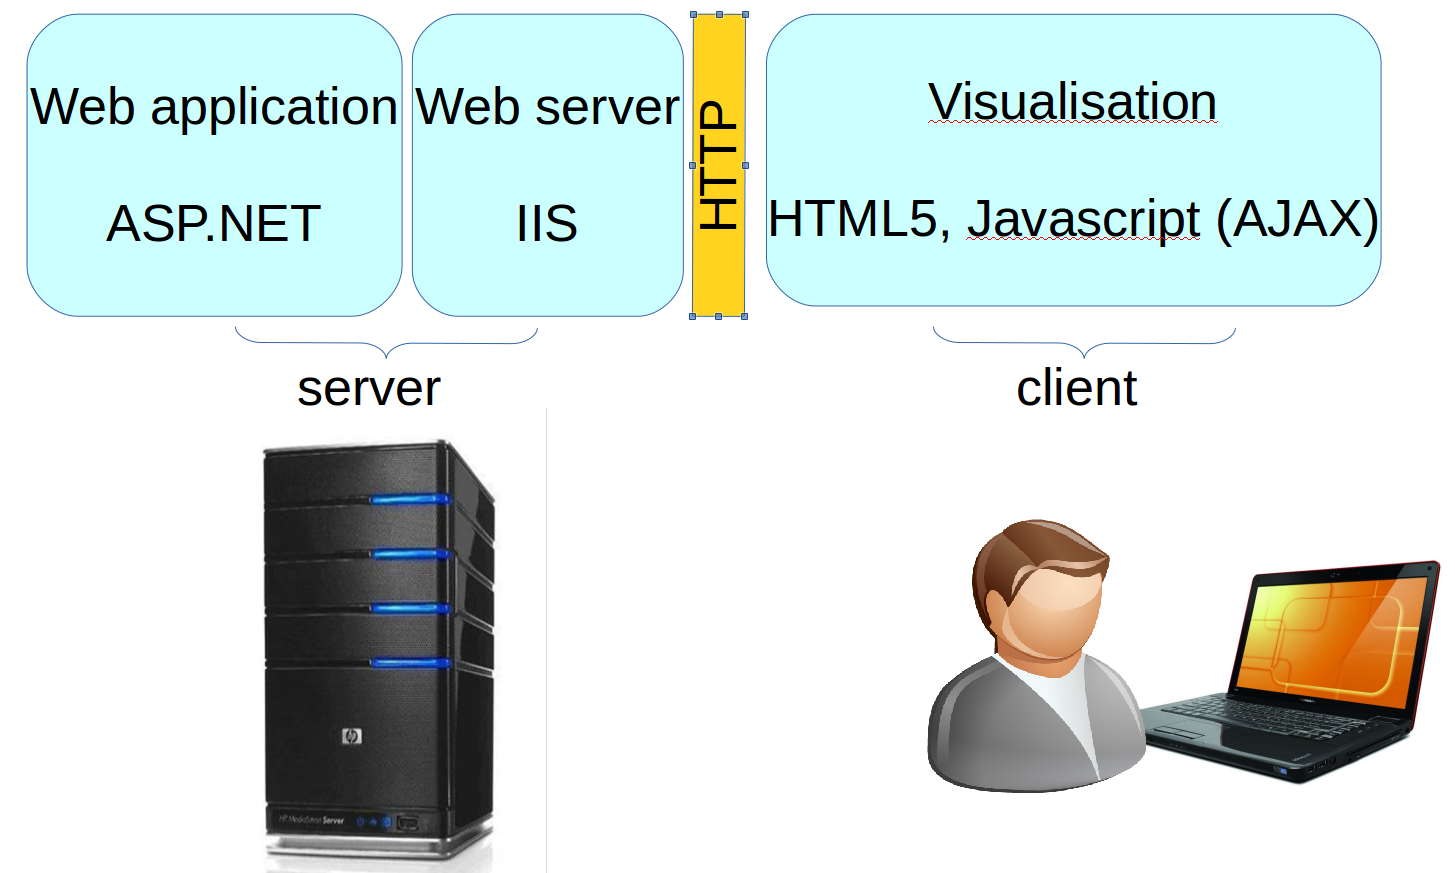
\includegraphics[width=1\textwidth]{chapter2/architektura.png}
    \caption{Example of client-server architecture involving web server which is middleware between web application and server platform. Client visualization in HTML5 web page communicates with server via HTTP protocol.}
    \label{fig:architecture}
\end{figure}

%Client-server architecture consist of two and more layers(tiers) E.g. three tier architecture consists of presentation (client) - logic and data tier (server) and each of the server tiers may reside on different physical resources. Example in fig. \ref{fig:architecture}) shows the web server, which is a middleware delivering some abstract functionality expected such as listening on specific TCP/UDP port, call appropriate functionality or deliver a static document, and such middleware is not implemented by the author of the application who deals only with server specific and client specific part. 

Service oriented architecture (SOA) is high level programming model based on self contained units of functionality. SOA introduces a new service layer in the client-server architecture which separate service interface from it's implementation. SOA principles and paradigms can be studied further in book of T. Erl. \cite{Erl2008}. 

Another approach represents objects and data of the system as resources with standard set of operations, create, read, update, delete (CRUD) and Representation State Transfer (REST) specifies several architectural constraints that helps scalability, performance and presents functionality via fixed number of operation and uniform resource location proposed by Fielding \cite{fielding2000chapter}. The REST style constraints towards the application is statelessness, resource orientated with uniform interface (CRUD) and hypermedia driven which should facilitate and optimize processing of resources via web based technologies, mainly HTTP protocol. 

While SOA focus on application design and easily turning the application objects into distributed services, REST is rather set of constraints to the architecture to handle the issues of distribution within web, as noted e.g. by Vinoski \cite{Vinoski2007}.

Software architecture of the enterprise application and distributed systems are studied in general and some repeating patterns are catalogued e.g. by Fowler et. al\cite{Fowler2003}. Integration patterns are discussed with focus on the ways of connecting heterogenous parts of the system as presents Hohpe et al.\cite{Hohpe2002}.
\subsubsection{Types of computing infrastructure}
When we focus on the architecture of the middleware and philosophy of building a computing infrastructure, these main types of distributed infrastructures are distinguished for scientific computing:
\begin{enumerate}
\item{\emph{Service grid-computing} is based on the idea that a computing resources (servers, clusters, special hardware) is owned by some organization but may be maintaned by some collective organization with an effort to provide a collection of services in best effort approach.}
\item{\emph{Desktop grid-computing} is based on the idea to connect generic desktop computers and provide the iddle computation time e.g. as a screen saver or background process to the projects.}
\item{\emph{Cloud-computing} provides architecture to services, platform or whole infrastructure in a way that an access to them is provided as a service with an impression of sole use it by user or process.
}
\end{enumerate}


\subsection{Service grid-computing}
\label{sec:servicegrid}

The Service-grid computing is based on a basic set of services implemented by a middleware to provide uniform interface for job scheduling and execution within the computing infrastructure. The term \emph{Grid} is used to emphasize the analogy with the electric power grid providing access to electricity \cite{foster2004}. Foster et al.\cite{foster2001,foster2004} and Chervenak et al. \cite{Chervenak2000} describe "data" and "computational" grid as shared hardware and software resources that provide reliable, consistent, pervasive and cheap access to high performance computational capacities and  effective and reliable execution of requests over data, which needs sensitive controlling of terabyte storages, data transfers to gigabits per seconds over global computer networks and scheduling such data transfer with respect to computational needs. The services provided by grid are either tools or web services following  \emph{Service Oriented Architecture}(SOA) for grid computing -- Open Grid Service Architecture (OGSA)\cite{Foster2003}. The security model and access to the grid infrastructure is proposed and implemented mainly by a mutual authentication between users and resources via public key infrastructure using X.509 certificate \cite{Foster1998}.

The fundamental part of any Grid is the computer network connecting resources that are distributed in different geographical location, generally Internet. 

The national grid initiative in Czech Republic 
-METACENTRUM\footnote{\url{http://www.metacentrum.cz} department of CESNET as national grid infrastructure} is interconnected via high-speed network CESNET 2 utilizing the technology of transfering data over optical cables using Dense wavelength division multiplexing (DWDM) \cite{novak2007deployment}. see fig. \ref{fig:cesnet} for further information.

\begin{figure}[ht]
    \centering
    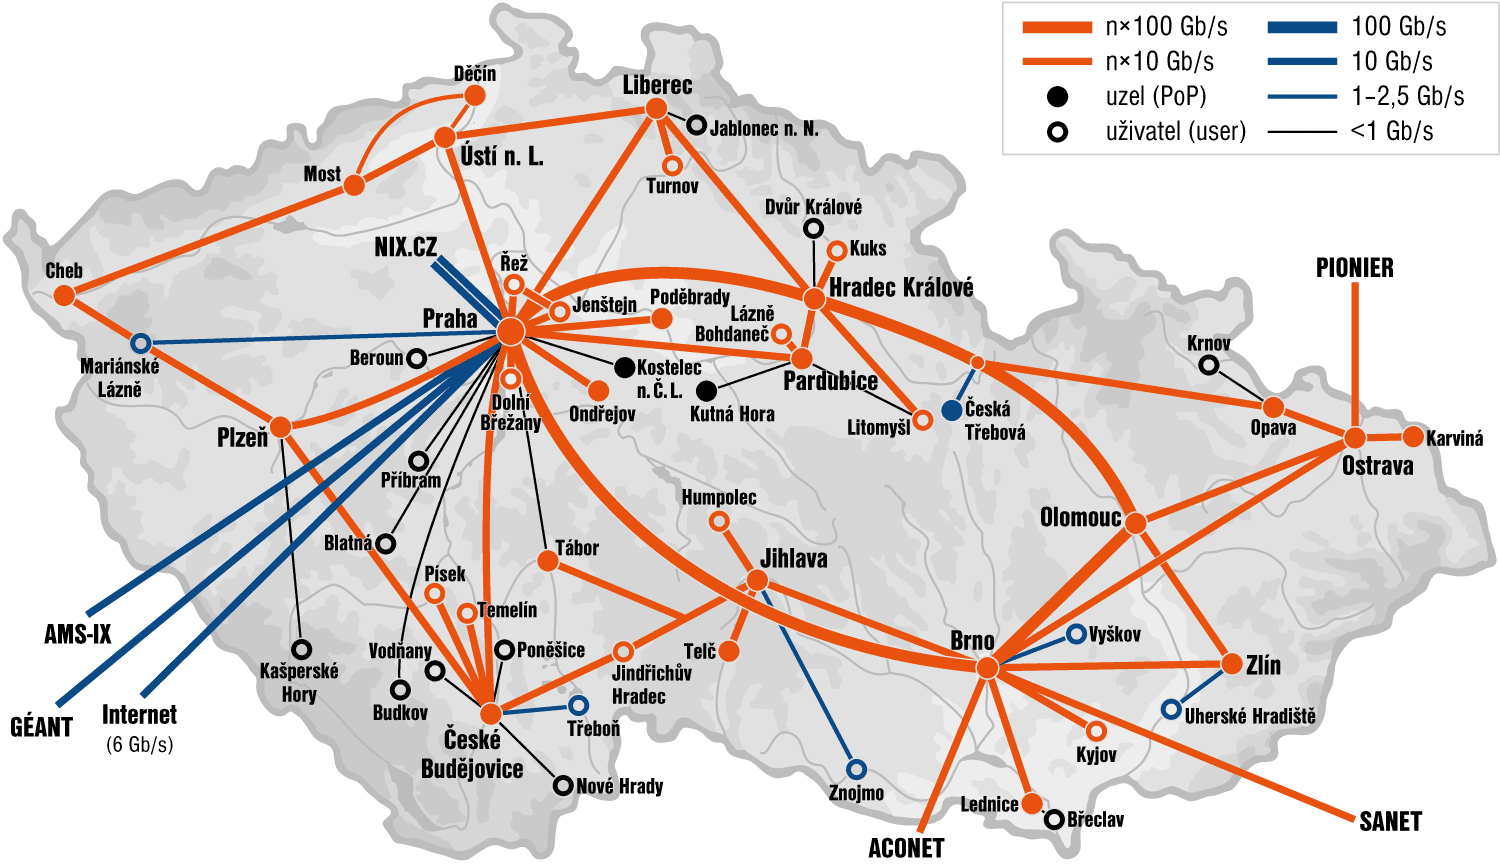
\includegraphics[width=1\textwidth]{chapter2/cesnet2-topo1.png}
    \caption{CESNET2 network topology as from december 2014 is maintaned by association of universities and academy of science CESNET. Interconnects mainly departments of universities and academy of sciences via rented physical network. It provides connection to general Internet via the czech NIX.cz (Neutral Internet eXchange), AMS-IX (Amsterdam Internet eXchange) and other channels to european research and education network GÉANT. Sources: \url{http://www.cesnet.cz}}
    \label{fig:cesnet}
\end{figure}

The administration and maintenance of such networked infrastructures are not trivial tasks and they are performed by experts of institutional computing centers or national laboratories and interconnected sites are managed and coordinated at national level or at international level. Such national organizations cooperate with similar national grid infrastructures in other countries. An umbrella organization in Europe --European Grid Infrastructure (EGI)\footnote{\url{http://www.egi.eu}}-- was established during 2010 and supports integration and coordination activities of NGI accross national boundaries with respect to the scientific collaboration which goes also across national boundaries. 

\begin{figure}[htb]
    \centering
    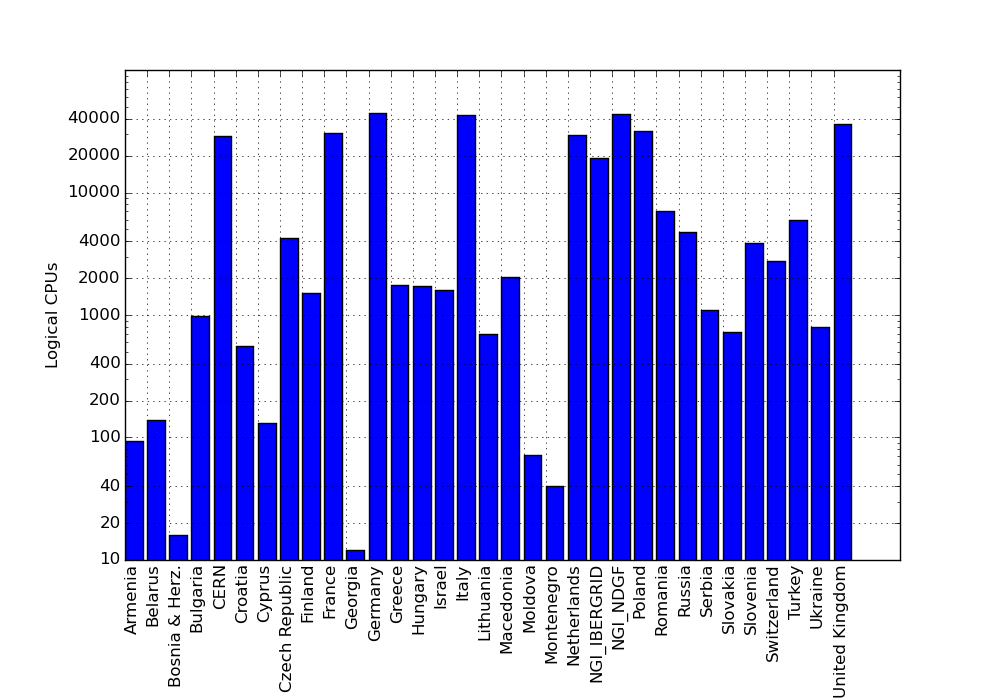
\includegraphics[width=1\textwidth]{chapter2/egicpus.png}
    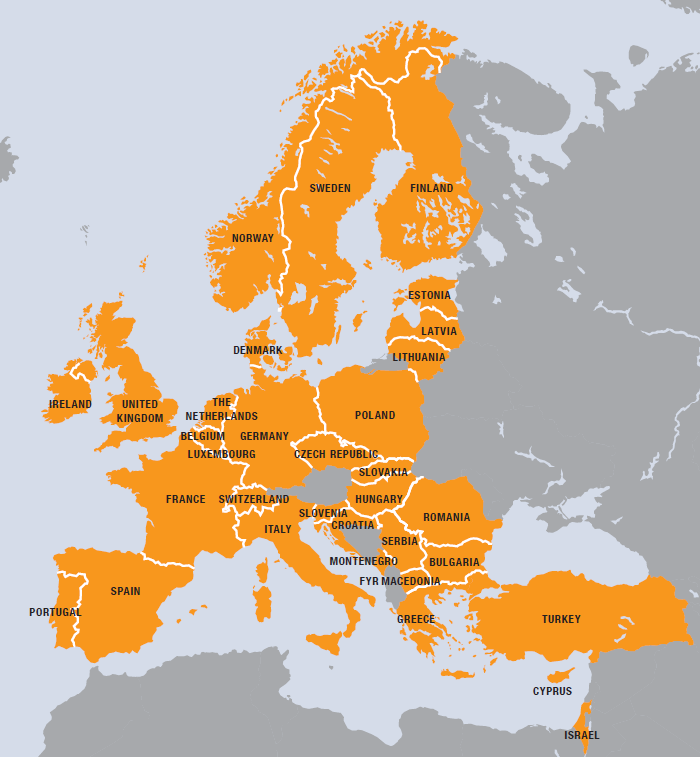
\includegraphics[width=0.6\textwidth]{chapter2/egi.png}
    \caption{Countries involved in EGI and number of CPUs within EGI infrastructure in 2012, the total logical CPU capacity at the end of 2012 was 349,720 cores( in graph per countries). CPU capacity was 433,957 cores in March 2014. Sources: EGI Compendium 2013, EGI statistics at \url{http://www.egi.eu}.%\bibentry{EGICompendium2013} \bibentry{egi2014}.
    }
    \label{fig:egi}
\end{figure}

The grow of several production grid infrastructure for science was accelerated in last decade mainly by the needs of experiments of high energy physics to process large number of observed data in a reasonable time \cite{Bird2009}. The Worldwide Large Hadron Collider Computing Grid (WLCG) has been designed to store and process almost 30 PetaBytes of data per year in the period of 2009-2013  \cite{Adamova2014} and is one of the largest grid deployed in the grid infrastructure. Other scientists from different scientific disciplines became users of this powerful infrastructure as well and with development of technologies, virtualization and cloud computing, the infrastructure may employ larger set of application and services and may become attractive for smaller scientific collaboration.

Several grid infrastructures were established based on different grid-middlewares.
Condor is one of the earliest effort to provide access to unutilized computers while preserving rights of the owners \cite{Litzkow1990}. glite \cite{Laure2006}\footnote{\url{http://glite.cern.ch}}, ARC\footnote{\url{http://www.nordugrid.org/arc/}} and Globus \cite{Foster1997}\footnote{\url{http://toolkit.globus.org/toolkit/}} are major grid-middleware operational in EGI.

Currently there is an effort to maintain interoperability between the infrastructures with different grid-middleware to reach the goal of shared world-wide grid \cite{Riedel2009}.

\subsection{Desktop grid-computing}
\label{sec:desktopgrid}
Joining desktop computers from an individual user to form a voluntary or desktop-grid was popularized by a project trying to identify uncommon signals from space to search extraterestrial intelligence (SETI@Home)\footnote{\url{http://setiathome.ssl.berkeley.edu/}}. It's based on the idea that a volunteer will download a small client program, which executes in background or instead of a screen saver; it downloads some ammount of raw data from a server on Internet to analyze and sends back the result to the server. In contrast to service grids, the authorization of users can't be so strong for volunteer individuals and some other policies, e.g. redundancy, is implemented to eliminate bad or cheating results \cite{Anderson2002}. After the success of the SETI@Home there were built general-purpose frameworks to facilitate development of projects that will use similar philosophy of computing on desktop computers connected via Internet such as BOINC  \cite{Anderson2004}, SZTAKI extension to BOINC \cite{Balaton2007,Kacsuk2009}, XtremWeb \cite{Fedak2001} and others. Currently there exists lot of similar projects gaining computer power as the SETI@Home project. E.g. the LHC@Home and it's successor LHC@Home 2 projects were established and used to execute some selected tasks of the LHC project on the desktop grid infrastructure \cite{Herr2006,Hoimyr2012}.

The desktop grids and service grids are two different approaches to gather computing power from large number of computing resources and e.g. the EdgE project achieved interoperability between these two worlds so the tasks using the first type of grid infrastructure can be scheduled in a second type of infrastructure \cite{Kacsuk2008,Urbah2009}.

\subsection{Virtualization}
\label{sec:introvirtual}
Virtualization technology separates the physical hardware layer from the software environment emulating a new virtual hardware layer. The hypervisor manages the guest virtual machines and translates the I/O from virtual device to physical device and instructions from virtual CPU to physical CPU. This introduces some overhead and performance degradation of virtual system compared to physical one. However, with recent virtualization technology introduced several techniques which reduces overhead and eliminate specific hardware features and instructions in OS which are hard to virtualize \cite{Barham2003,Youseff2006}.
Thanks to them, a virtual environment fine tuned for an application can be executed on almost any hardware and platform and virtualization becomes part of the solution to execute jobs of desktop-grid or service-grid computation on different physical platforms \cite{ruda2009virtual}.
Currently there exists several commercial, free or even opensource virtualization implementation which are provided by different vendors and it's hypervisor - VMWare, XEN, KVM, VirtualBox etc. And several vendors provides provisioning of virtual infrastructure for computing which are now distinguished as cloud-computing.

\subsection{Cloud computing}

In contrast to grid-computing where user scheduled jobs accessing shared environment and might be influenced by other users or by the environment, the cloud-computing provides access to a virtual software, platform or whole infrastructure so the user or process has impression of sole use. Virtualization techniques enabled expansion of cloud-computing mainly on infrastructure which was built for another purpose and can be rented in times when the primary infrastructure is not fully utilized \cite{Foster2008}. 

Cloud-computing can be characterized as "a model for enabling ubiquitous, convenient, on-demand network access to a shared pool of configurable computing resources (e.g., networks, servers, storage, applications, and services) that can be rapidly provisioned and released with minimal management effort or service provider interaction."  \cite{Mell2011}.  

Cloud computing makes computational power and storage as utility or commodity that can be rented. It evolves in commercial area to facilitate scaling up the business needs with computational demand with current commercial clouds such as Amazon EC\footnote{\url{http://aws.amazon.com/ec2/}}, Microsoft Windows Azure \footnote{\url{http://azure.microsoft.com/}}, Google cloud\footnote{\url{https://cloud.google.com/}} and others.

Cloud computing in research infrastructures were recently deployed next to the already existing grid-infrastructures and utilizes the same hardware resources. Some methods to integrate grid-computing and cloud computing were introduced \cite{Anjum2012}. Access is provided to the same users of grid-infrastructure and currently most used platforms are Open\-Nebula  \cite{Milojicic2011} and OpenStack  \cite{Kumar2014}.

An interoperability among cloud providers and standardization on cloud-computing, virtualization and related technologies is important as it would keep users from being locked into a specific cloud provider\cite{Ortiz2011}.

\subsection{Application model}

The application computed within grid or cloud can be characterized by the quantity of tasks being performed, the size of input data and of the communication needs to be done between concurrent tasks. 
Grid-computing infrastructures were primarily utilized for computation, which tasks take long time, were relatively loose coupled and resources were used over long period of time. Performance/capacity is usually mentioned  in operations/CPUs per month or year and for such computation the term High throughput computing (HTC) is used.

While HTC takes long time, the High Performance Computing (HPC) is usually characterized by computing the problems which have small number of tasks and are relatively tightly coupled and can be executed in highly parallel environment. Performance is measured usually in operations per second  \cite{Hager2010,Levesque2010}. The grid infrastructure can involve HPC servers or clusters, thus a job or tasks that requires such HPC hardware are scheduled and executed there.

Many Task Computing(MTC) aims to bridge HTC and HPC, while the computation usually takes shorter time, the data exchange is in MB rather in GB, performance is measured in tasks per seconds rather than jobs per months or years and involves computing relatively much more heterogenous problems which are not "happily" parallel. However, middleware for HPC or HTC which are present in grid-computing infrastructures may introduce some shortcomings, therefore a prototype task execution framework suitable for MTC was proposed and implemented \cite{Raicu2008, Raicu2009,Raicu2010}.
The MTC seems suitable to be performed on cloud-computing technologies, which introduces some benefits over classical grids, however such clouds should be oriented for HPC systems and generic public cloud may introduce low performance than expected \cite{Iosup2010}.

\subsection{Workflows and Gateways}
\label{sec:introworkflow}
A workflow is an abstract description of the process of computation and data manipulation specified by an expert to express what should be done within the distributed system. It automates the process of computation by composing data manipulation steps and tasks and solving failure events.

The workflow can be encoded in any programming or scripting language, however some higher level languages evolved. In business domain a Business Process Execution Language (BPEL) is an OASIS standard and becomes one of the most used language for describing workflow of orchestration of web services and transaction steps \cite{Pasley2005}. In scientific domain different workflow systems are operational including BPEL with different capabilities. Taxonomies of some existing workflow systems were published by Yu, Zhao et al. \cite{Yu2005a,Zhao2008,Curcin2008}. Workflows in cloud computing are covered by web technologies programming languages (Javascript) \cite{Foster2008}.

The workflow system which implements the concrete workflow language is usually tightly coupled with the specific grid-computing or cloud-computing infrastructure. 

To connect different grid-infrastructures a mutual workflow management system is used to integrate them as proposed by Kacsuk et al. \cite{Kacsuk2008a,Kacsuk2011} or an interoperability is solved by separating abstract workflow representation and concrete implementation showed on selected existing workflow systems introduced by Planensteiner et al. \cite{Plankensteiner2013}.

Scientific gateway incorporates higher level services for specific scientific community e.g. as a web portal or desktop application to control the process of computation via a workflow\cite{Wilkins-Diehr2007}. For building the scientific gateways several frameworks were developed e.g. Apache Airavata \cite{Pierce2014,Memon2014} or WS-PGRADE/gUSE\cite{Kacsuk2012}. And the concrete instances are available for broader area of scientific community. 


%\section{Informatics in Medicine and Biology}
%\label{sec:biology}

